\begin{figure}[htbp]\centering
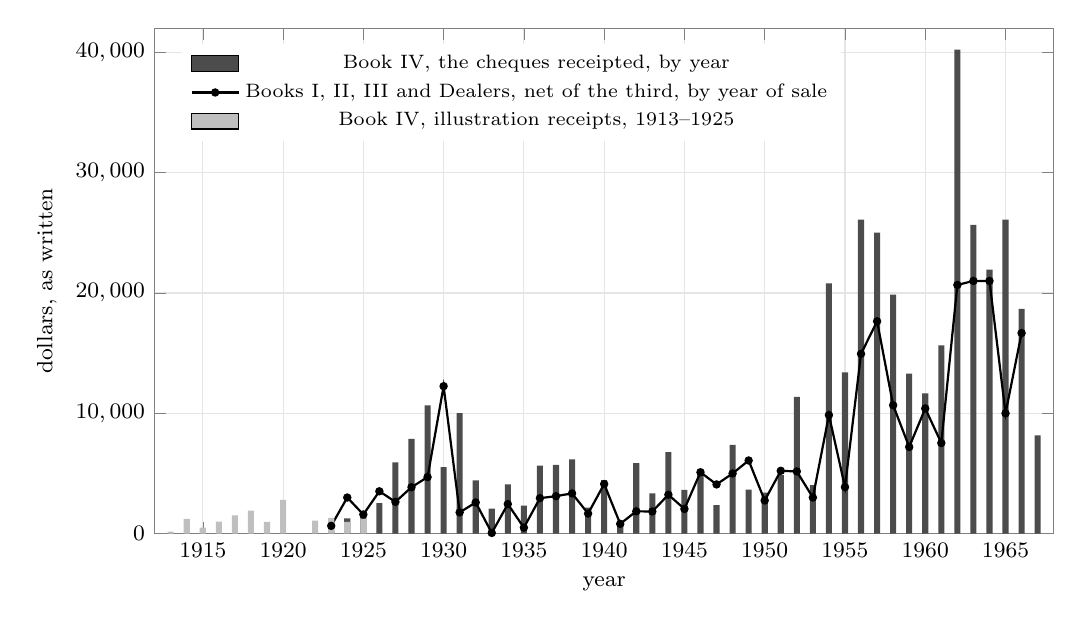
\begin{tikzpicture}
\begin{axis}[width=13cm,height=8cm,xmin=1912,xmax=1968,ymin=0,ymax=42000,xlabel={year},ylabel={dollars, as written},grid=major,grid style={black!10},tick label style={font=\footnotesize},label style={font=\footnotesize},axis line style={black!50},legend style={font=\scriptsize,at={(0.03,0.97)},anchor=north west,draw=none},scaled y ticks=false,y tick label style={/pgf/number format/fixed,/pgf/number format/1000 sep={,}},x tick label style={/pgf/number format/1000 sep=}]
\addplot[ybar,bar width=2.2pt,fill=black!70,draw=none,area legend] coordinates {(1920,71) (1922,141) (1923,301) (1924,1260) (1925,1528) (1926,2528) (1927,5918) (1928,7871) (1929,10661) (1930,5533) (1931,10019) (1932,4422) (1933,2081) (1934,4087) (1935,2334) (1936,5640) (1937,5714) (1938,6171) (1939,2160) (1940,4438) (1941,875) (1942,5857) (1943,3338) (1944,6762) (1945,3632) (1946,5342) (1947,2361) (1948,7375) (1949,3661) (1950,3408) (1951,4870) (1952,11371) (1953,4029) (1954,20800) (1955,13406) (1956,26099) (1957,25013) (1958,19861) (1959,13290) (1960,11657) (1961,15637) (1962,40218) (1963,25657) (1964,21948) (1965,26100) (1966,18667) (1967,8157)};
\addlegendentry{Book IV, the cheques receipted, by year}
\addplot[thick,black,mark=*,mark size=1.1pt] coordinates {(1923,647) (1924,3000) (1925,1590) (1926,3517) (1927,2637) (1928,3855) (1929,4698) (1930,12252) (1931,1765) (1932,2587) (1933,57) (1934,2453) (1935,500) (1936,2947) (1937,3113) (1938,3342) (1939,1667) (1940,4121) (1941,813) (1942,1853) (1943,1840) (1944,3233) (1945,2053) (1946,5100) (1947,4087) (1948,5000) (1949,6077) (1950,2753) (1951,5220) (1952,5167) (1953,3000) (1954,9853) (1955,3867) (1956,14940) (1957,17647) (1958,10667) (1959,7200) (1960,10400) (1961,7530) (1962,20667) (1963,21000) (1964,21000) (1965,10000) (1966,16667)};
\addlegendentry{Books I, II, III and Dealers, net of the third, by year of sale}
\addplot[ybar,bar width=2.2pt,fill=black!25,draw=none,area legend] coordinates {(1913,160) (1914,1225) (1915,500) (1916,991) (1917,1514) (1918,1916) (1919,977) (1920,2794) (1922,1075) (1923,1304) (1924,980) (1925,1219)};
\addlegendentry{Book IV, illustration receipts, 1913--1925}
\end{axis}
\end{tikzpicture}
\caption{The money, three ways: what the pocket book receipts each year from 1920 (dark bars), what the work books state as the net of sales dated in that year (line), and the illustration receipts of the first decade (pale bars). The two art series are not the same number and should not be: one is the dealer's cheques as they arrived, the other the studio's record of what left. Every figure is a floor, read from the transcribed rows under the rules of the accounts chapter. After the Accounts tab of hopper.commutator.io. Drawn by Claude Fable~5.1, 13 September 2026, from \texttt{accounts.json} (2026-09-19).}\label{fig:money}
\end{figure}
